\documentclass{standalone}
\usepackage{tikz}
\begin{document}
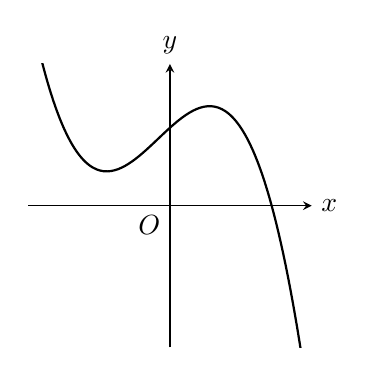
\begin{tikzpicture}[>=stealth, scale=0.9]
  % Axes
  \draw[->] (-2,0) -- (2,0) node[right] {$x$};
  \draw[->] (0,-2) -- (0,2) node[above] {$y$};
  \node[below left] at (0,0) {$O$};

  % Function curve: steep descent from upper-left, local min in QII,
  % local max in QI above x-axis, then descends crossing the x-axis.
  \begin{scope}
    \clip (-2,-2) rectangle (2,2);
    \draw[thick]
      plot[smooth, domain=-2.5:2.5, samples=100]
        (\x, {-0.6*\x*\x*\x - 0.3*\x*\x + 0.9*\x + 1.1});
  \end{scope}
\end{tikzpicture}
\end{document}
